\documentclass[12pt,a4paper]{article}
\usepackage{amsmath,amscd,amsbsy,amssymb,latexsym,url,bm,amsthm}
\usepackage{epsfig,graphicx,subfigure}
\usepackage{enumitem,balance}
\usepackage{wrapfig}
\usepackage{mathrsfs,euscript}
\usepackage[usenames]{xcolor}
\usepackage{hyperref}
\usepackage[vlined,ruled,linesnumbered]{algorithm2e}
\hypersetup{colorlinks=true,linkcolor=black}

\newtheorem{theorem}{Theorem}
\newtheorem{lemma}[theorem]{Lemma}
\newtheorem{proposition}[theorem]{Proposition}
\newtheorem{corollary}[theorem]{Corollary}
\newtheorem{exercise}{Exercise}
\newtheorem*{solution}{Solution}
\newtheorem{definition}{Definition}
\theoremstyle{definition}

\renewcommand{\thefootnote}{\fnsymbol{footnote}}

\newcommand{\postscript}[2]
 {\setlength{\epsfxsize}{#2\hsize}
  \centerline{\epsfbox{#1}}}

\renewcommand{\baselinestretch}{1.0}

\setlength{\oddsidemargin}{-0.365in}
\setlength{\evensidemargin}{-0.365in}
\setlength{\topmargin}{-0.3in}
\setlength{\headheight}{0in}
\setlength{\headsep}{0in}
\setlength{\textheight}{10.1in}
\setlength{\textwidth}{7in}
\makeatletter \renewenvironment{proof}[1][Proof] {\par\pushQED{\qed}\normalfont\topsep6\p@\@plus6\p@\relax\trivlist\item[\hskip\labelsep\bfseries#1\@addpunct{.}]\ignorespaces}{\popQED\endtrivlist\@endpefalse} \makeatother
\makeatletter
\renewenvironment{solution}[1][Solution] {\par\pushQED{\qed}\normalfont\topsep6\p@\@plus6\p@\relax\trivlist\item[\hskip\labelsep\bfseries#1\@addpunct{.}]\ignorespaces}{\popQED\endtrivlist\@endpefalse} \makeatother

\begin{document}
\noindent

%========================================================================
\noindent\framebox[\linewidth]{\shortstack[c]{
\Large{\textbf{Lab03-Greedy Strategy}}\vspace{1mm}\\
CS214-Algorithm and Complexity, Xiaofeng Gao, Spring 2021.}}


\begin{center}
\footnotesize{\color{red}$*$ If there is any problem, please contact TA Haolin Zhou.}\par
% Please write down your name, student id and email.
\footnotesize{\color{blue}$*$ Name:\underline{Xin Xu}  \quad Student ID:\underline{519021910726} \quad Email: \underline{xuxin20010203@sjtu.edu.cn}}
\end{center}

\begin{enumerate}
	\item \textit{Interval Scheduling.} Interval Scheduling is a classic problem solved by \textbf{greedy algorithm}: given $n$ jobs and the $j$-th job starts at $s_j$ and finishes at $f_j$. Two jobs are compatible if they do not overlap. The goal is to find maximum subset of mutually compatible jobs. Tim wants to solve it by sort the jobs in descending order of $s_j$. Is this attempt correct? Prove the correctness of such idea, or else provide a counter-example.
	    \begin{solution}
	        No. This attempt isn't correct for the job with an earlier starting time may have a later finishing time, too. The counter-example is below.
			\begin{figure}[htbp]
                \centering
                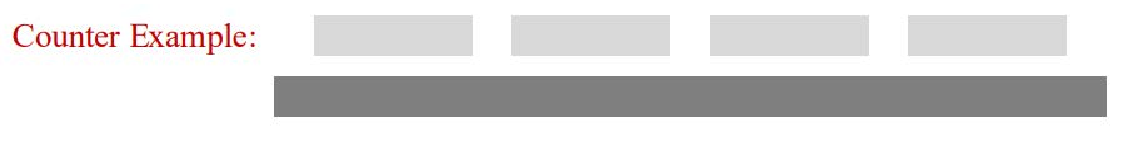
\includegraphics[width=0.4\textwidth]{counter-example.pdf}
                \caption{The Counter Example}\label{counter-example}
            \end{figure}
	    \end{solution}
	
	\item \textit{Done deal.} In a basketball league, teams need to complete player trades through matching contracts. Every player is offered a contract. For the sake of simplicity, we assume that the unit is $ M $, and the size of all contracts are integers. The process of contract matching refers to the equation: $ \sum_{i\in A} a_{i}=\sum_{j\in B} b_{j} $, where $ a_{i} $ refers to the contract value of player $ i $ in team $A$ involved in the trade and $ b_{j} $ refers to the value of player $ j $ in team $B$. 
	
	Assume that you are a manager of a basketball team and you want to get \textbf{one} star player from another team through trade. The contract of the star player is $ n (n\in \mathbb{N}^+) $. The goal is to complete the trade with as few players as possible. 
	
	\begin{enumerate}
		\item Describe a \textbf{greedy} algorithm to get the deal done with the least players in your team. Assume that there are only 4 types of contracts in your team: $25M$, $ 10M $, $ 5M $, $ 1M $, and there is no limit to the number of players. Prove that your algorithm yields an optimal solution.
		\item Suppose that the available contract sizes are powers of $c$,
		i.e., the values are $c^{0}, c^{1}, \ldots, c^{k}$ for some integers $c>1$ and $k \geq 1$. Show that the greedy algorithm always yields an optimal solution.
		\item Give a set of contract sizes for which the greedy algorithm does not yield an optimal solution. Your set should include a $ 1M $ so that there is a solution for every value of $ n $.
	\end{enumerate}
    \begin{solution}
        \begin{enumerate}
			\item We can apply a greedy algorithm recursively. Suppose the value of the star player is $x$ and the $4$ types of contracts in an increasing order are $c_1,c_2,c_3,c_4$. For every $c_k \leqslant x< c_{k+1}$, we choose the contract with value of $c_k$ and recursively apply this method to $x-c_k$ untill the remainder is zero.
			      \\We will prove this algorithm is optimal by contradiction. If the greedy algorithm isn't optimal, and there is another optimal method, which quiz to choose $c_k$ for the condition that $c_k \leqslant x< c_{k+1}$. In this case, it must choose $c_1,c_2,...,c_{k-1}$ to meet the value of $c_k$. If $c_k=25M$, there are at least three contracts with values of $\{10M,10M,5M\}$. If $c_k=10M$, there are at least two contracts with values of $\{5M,5M\}$. If $c_k=5M$, there are at least five contracts with values of $\{1M,1M,1M,1M,1M\}$.
				  Considering all conditions, the number of contracts are all larger than one. And we can figure out a more optimal method by replacing the chosen contracts with the one that greedy algorithm picks, which is contract to our hypothesis. So, the greedy algorithm is optimal.
			\item We can easily get the idea that in an optimal method, the number of all the contracts is less than $c$ except the one with largest value because for any number $\geqslant c$, we can replace $c$ contracts of that value with just one contract of the higher value. So, we can prove it by contradition. If we don't choose $c^k$ in the situation that $c^k \leqslant x< c^{k+1}$, we can only choose $(c-1)c^{k-1}+(c-1)c^{k-2}+...+(c-1)c^{2}+(c-1)c^{1}$, whose sum is just $c^k-1$. To meet up the value of $c^k$, we must choose one more contract, which is contrast to our observation.
			      So, the greedy algorithm is an optimal solution in this case.
			\item The set of contract sizes are $\{50M,35M,10M,1M$\}. In this case, if we want to get a contract with the value of $70M$, greedy algorithm picks $\{50M,10M,10M\}$ while the optimal method is to pick $\{35M,35M\}$.
		\end{enumerate}
    \end{solution}
	
    \item \textit{Set Cover.} \textbf{Set Cover} is a typical kind of problems that can be solved by greedy strategy. One version is that: Given $n$ points on a straight line, denoted as $\{x_i\}_{i=1}^n$, and we intend to use minimum number of closed intervals with fixed length $k$ to cover these $n$ points.
    \begin{enumerate}
    	\item Please design an algorithm based on \textbf{greedy} strategy to solve the above problem, in the form of \emph{pseudo code}. Then please analyze its \emph{worst-case} complexity.
    	\item Please prove the correctness of your algorithm.
    	\item Please complete the provided source code by C/C++ {\color{blue}(The source code \emph{Code-SetCover.cpp} is attached on the course webpage)}, and please write down the output result by testing the following inputs: 
    	\begin{enumerate}
    		\item the number of points $n=7$;
    		\item the coordinates of points
    		$x=\{1,2,3,4,5,6,-2\}$;
    		\item the length of intervals
    		$k=3$.
    	\end{enumerate}
        \textbf{Remark}: Screenshots of running results are also acceptable 
    \end{enumerate}
    \begin{solution}
        \begin{enumerate}
			\item The pseudo code is below.
			\\\begin{algorithm}[H]
				\KwIn{An array $x[1,\cdots,n]$, the number of points $n$, and the length of intervals $k$.}
				\KwOut{The minimum number of closed intervals with fixed length $k$ to cover these $n$ points.}
				
				\BlankLine
				\caption{Greedy}\label{Alg-greedy}
	
				Sort $n$ points by values so that $x_1< x_2<...<x_{n-1}<x_n$\;
				$i\leftarrow 2$;$num\leftarrow 1$;$start\leftarrow x_1$;$end\leftarrow start+k$\;
				\While{$end<x_n$}{
					\While{$end\geqslant x_i$}{
						$++i$\;
					}
					$start\leftarrow x_i$\;
					$end\leftarrow x_i+k$\;
					$++num$\;
				}
				
				\Return $num$\;

			\end{algorithm}

            \textbf{Time Complexity.} In worst case, the time complexity of sorting is $O(n^2)$ and the time complexity of the while-loop is $O(n)$. So, the time complexity of worst case is $O(n^2)$.
			\item 
			\begin{proof}
				We will prove the greedy algorithm by contraction. In the greedy algorithm, each interval starts at an exact point in such as $x_i$. And if an interval starts before $x_i$ but doesn't reach the point $x_{i-1}$, we can move it to $x_i$ which doesn't decrease the number of points that interval covers,
				but may increase it. So, suppose there is an another optimal method with the max number of intervals starting exactly at $x_i$, which we assume as $r$. We can replace exceptional intervals with ones creating by greedy algorithm. And this action leads to at least as optimal method as former one, which is contrast to our hypothesis that the max number is $r$.
				So, the greedy algorithm is optimal.
			\end{proof}
			\item The .cpp file is in the folder, and the result is 3.
		\end{enumerate}
    \end{solution}

\end{enumerate}



\vspace{20pt}

\textbf{Remark:} You need to include your .pdf and .tex files in your uploaded .rar or .zip file.

%========================================================================
\end{document}
